
\documentclass[]{article}

\title{Distribución de probabilidad de normal }

\date{}
\usepackage{braket}
\usepackage{bbold}
\usepackage{amsmath,amsfonts,amssymb,amsthm,booktabs}
\usepackage[margin=1.0in]{geometry}
\usepackage{graphicx}
\usepackage{chngcntr}
\usepackage{floatrow}
\usepackage{chngcntr}
\usepackage{hyperref}
\usepackage[spanish]{babel}
\usepackage[svgnames]{xcolor}
\usepackage{listings}
\usepackage[%
    font={small,sf},
    labelfont=bf,
    format=hang,    
    format=plain,
    margin=0pt,
    width=0.8\textwidth,
]{caption}
\usepackage[list=true]{subcaption}
\lstset{language=R,
    basicstyle=\small\ttfamily,
    stringstyle=\color{DarkGreen},
    otherkeywords={0,1,2,3,4,5,6,7,8,9},
    morekeywords={TRUE,FALSE},
    deletekeywords={data,frame,length,as,character},
    keywordstyle=\color{blue},
    commentstyle=\color{DarkGreen},
}

\counterwithin{figure}{section}
\renewcommand*{\figureautorefname}{Figura}


\usepackage[backend=biber]{biblatex}
\addbibresource{ref.bib}
\begin{document}
	\maketitle
	\begin{center}


\centerline{\textbf{TAREA 5} } 
\textbf{ }

\centerline{Alumno: } 
\centerline{Joaquín Arturo Velarde Moreno}


	\end{center}
	

\section{Introducción}
En el siguiente reporte vamos a definir el comportamiento de una distribución normal, ver sus formulas y sus representaciones en histogramas, haremos uso del programa R 4.0.2 \cite{rproject} para hacer cálculos con conjuntos de datos y mostrarlos gráficamente usando como apoyo el material de la Doctora Elisa Schaefer \cite{rproject}.
También intentaremos simular una distribución normal a partir de valores uniformes utilizando la transformada de box-Muller.
\section{Definición}
la distribución normal o Gaussiana, nombrada así por Gauss, es una distribución usada para aproximarse al valor de una variable aleatoria continua a una situación ideal. Esta consiste de 2 parámetros $\mu$ y $\sigma$.
donde:
\begin{itemize}
	\item $\mu$ es la media de la distribución.
	\item $\sigma$ es la desviación estándar.
\end{itemize}
si sacáramos una encuesta de la edad de cada uno de los 150 estudiantes de una escuela y obtuviéramos que su promedio es de 18 años, tendríamos un histograma donde se empieza a ver que hay una mayor cantidad de alumnos cerca del promedio a la media \autoref{fig:Negativo}, esto da la tendencia de querer aproximarse a una curva de distribución normal \autoref{fig:Densidad} .

Si a esto lo aproximamos a una situación ideal no tomando solo 150 si no tomando la de 5000 estudiantes entonces veremos mas fácilmente la forma de nuestra distribución acercándose a la curva de la distribución normal \autoref{fig:Regular}, esta curva nos indica 2 cosas sobre esta distribución.

 \textbf{Asimétrica} significa que la media es igual a los valores de la moda y la mediana, en otras palabras los alumnos que estén mas cerca del promedio son mas numerosos que los que están mas alejados de este promedio, esto también implica que se cumple la siguiente ecuación.
 
\[f_X(\mu - x) = f_X(\mu + x) \, \forall x\in \mathbb{R} \]

  
\textbf{Asintotica} Que se acerca continuamente a la recta de los eje x sin llegar nunca a encontrarla, es decir puede extenderse hasta el infinito.


 la desviación estándar se representa con la letra griega $\sigma$ (sigma), y nos indica lo lejos que están distribuidos los resultados de la media, esto puede producir 2 situaciones una situación homogénea o heterogénea.
 
Si la situación es homogénea la desviación $\sigma$ es muy reducida y los sujetos están todos muy cercanos a la media $\mu$ y la curva será muy afilada \autoref{fig:Regular}.
En cambio si la situación es heterogénea la desviación $\sigma$ es muy alta y los sujetos están todos muy alejados a la media $\mu$ y la curva sera menos afilada \autoref{fig:Heterogenea}.

\section{Formula}
La formula para la función de probabilidad normal esta definida por la siguiente expresión
\[f_X(x) = \frac{1}{\sigma \sqrt{2\pi }}exp^{(\frac{-(x-\mu)^{2}}{2\sigma^{2} })}\]

donde:
\begin{itemize}
	\item $\mu$ es la media de la distribución.
	\item $\sigma$ es la desviación estándar.
\end{itemize}
 Esta ecuación es demasiado complicada incluso para hacerlo en calculadora, para este tipo de cálculos se suele hacer uso de la herramienta R \cite{rproject} , en el cual ya esta predefinido con la siguiente función \textit{dnorm()}, y si queremos
generar un vector de una distribución normal podemos utilizar
el método \textit{rnorm()}.
  \begin{lstlisting}

    Promedio <- 18
    Edad     <- rnorm(500000,Promedio,1)
   \end{lstlisting}

 si lo graficamos con histograma tendremos la misma distribución normal que se espera \autoref{fig:Regular}
\section{Método de Box-Muller}
También podemos generar una distribución normal por otros métodos tales como el método de Box-Muller el cual es un método de generación de pares de números aleatorios independientes con distribución normal estándar, es decir con esperanza cero y varianza unitaria, expresada en las siguientes formulas.
\[Z_{0} = R\, cos(\Theta ) = \sqrt{-2\, log(U_{1})}\,  cos(2\pi\,  U_{2})\]
\[Z_{1} = R\, sin(\Theta ) = \sqrt{-2\, log(U_{1})}\,  sin(2\pi\,  U_{2})\]

donde:
\begin{itemize}
	\item $U_{1}\, y\, U_{2}$ son variables aleatorias independientes con una distribución uniforme entre los valores 0 a 1.
	\item $Z_{1}\, y\, Z_{2}$ son variables aleatorias independientes con un distribución normal con una desviación estándar de 1.
\end{itemize}

Esto expresado en R puede ser definido como :
  \begin{lstlisting}
    u = runif(2);
    z0 = sqrt(-2 * log(u[1])) * cos(2 * pi * u[2]);
    z1 = sqrt(-2 * log(u[1])) * sin(2 * pi * u[2]);
   \end{lstlisting}
Si queremos tener nuestra propia media y desviación podemos afectar la variable aleatoria.
  \begin{lstlisting}
    mu      = 18;
    sigma   = 1;
    u       = runif(2);
    z0      = sqrt(-2 * log(u[1])) * cos(2 * pi * u[2]);
    z1      = sqrt(-2 * log(u[1])) * sin(2 * pi * u[2]);
    z0      = sigma * z0 + mu);
    z1      = sigma * z1 + mu);
   \end{lstlisting}
Si utilizamos este método para generar nuestras variables aleatorias obtendríamos que son similares a la distribución normal \autoref{fig:foobar}. 


Es necesario que ambas funciones se obtengan al calcular con 2 variables aleatorias de distribución uniforme, en el caso de cambiar el calculo usando solo una sola variable uniforme, rompería la distribución normal \autoref{fig:singlevariable} .
Esto lo podemos verificar con el método \textit{Shapiro.test()}
el cual nos devuelve un valor \textit{p-value}, si el valor obtenido es mayor a 0.05 entonces significa que nuestro vector muy probablemente viene de una distribución normal, sin embargo este método solo puede trabajar con un vector de 1 a 5000 valores, debido a esto es bueno utilizar el método \textit{sample()} para tratar con vectores muy grandes.
  \begin{lstlisting}
    test <- shapiro.test(runif(100)) 
    print(test)
    data:  runif(100)
	W = 0.95081, p-value = 0.0009379
	
	# prueba negativa 0.0009379 < 0.05
	                 
    test <- shapiro.test(sample(Edades, 5000, replace = TRUE))
    print(test)
	data:  sample(Edades, 5000, replace = TRUE)
	W = 0.99963, p-value = 0.5049
	
	# prueba positiva 0.5049 > 0.05
   \end{lstlisting}



\begin{figure}[b]
    \centering
    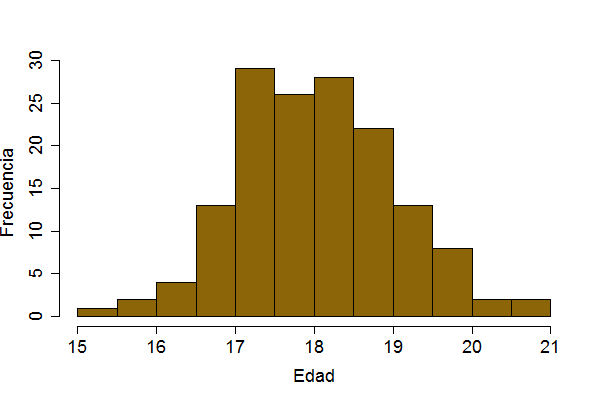
\includegraphics[width=.5\linewidth]{Frecuencia.png}    \caption{Distribución de frecuencia de la encuesta.}
    \label{fig:Negativo}
\end{figure}

\begin{figure}[b]
    \centering
    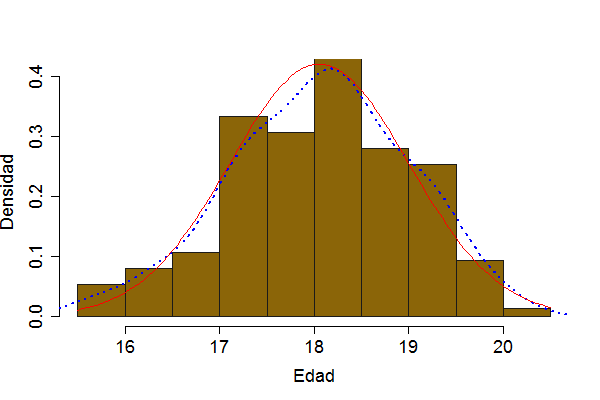
\includegraphics[width=.5\linewidth]{Densidad.png}    \caption{Densidad de resultados en la encuesta.}
    \label{fig:Densidad}
\end{figure}

\begin{figure}[b]
    \centering
    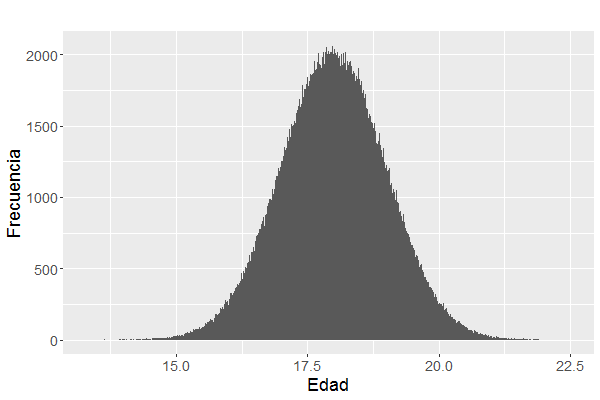
\includegraphics[width=.5\linewidth]{Ideal.png}    \caption{Distribución de frecuencia de la encuesta con 50000 estudiantes.}
    \label{fig:Regular}
\end{figure}

\begin{figure}[b]
    \centering
    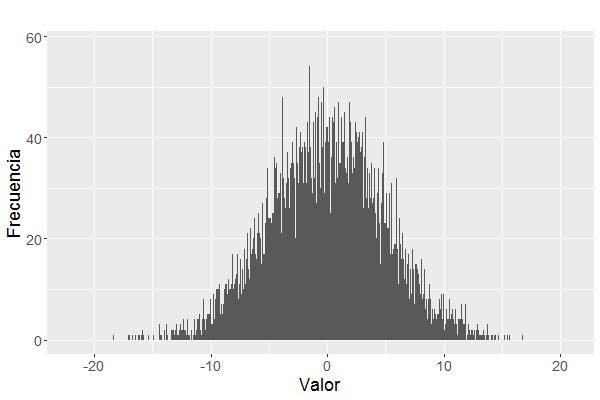
\includegraphics[width=.5\linewidth]{Heterogenea.png}    \caption{Distribución de frecuencia normal heterogénea.}
    \label{fig:Heterogenea}
\end{figure}





\begin{figure}
\centering
\subcaptionbox{Distribución de frecuencia con una sola variable $Z_{1}$.}{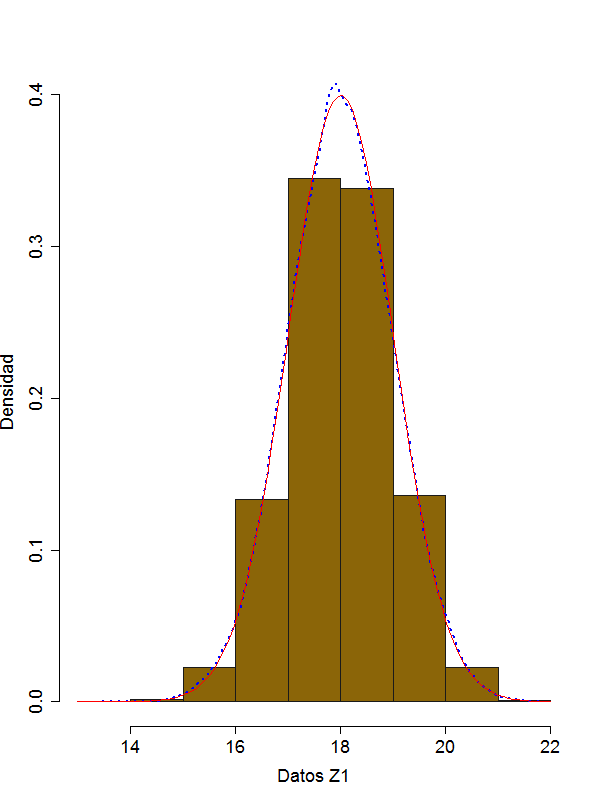
\includegraphics[width=0.3\textwidth]{BoxMuller_z1.png}}%
\hfill
\subcaptionbox{Distribución de frecuencia con una sola variable $Z_{0}$.}{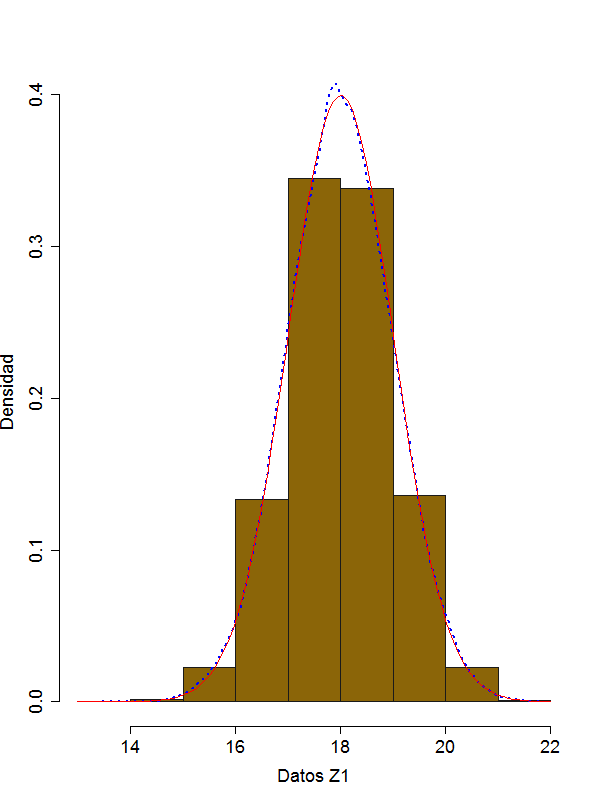
\includegraphics[width=0.3\textwidth]{BoxMuller_z1.png}}%
\hfill
\subcaptionbox{Distribución de frecuencia con ambas variables.}{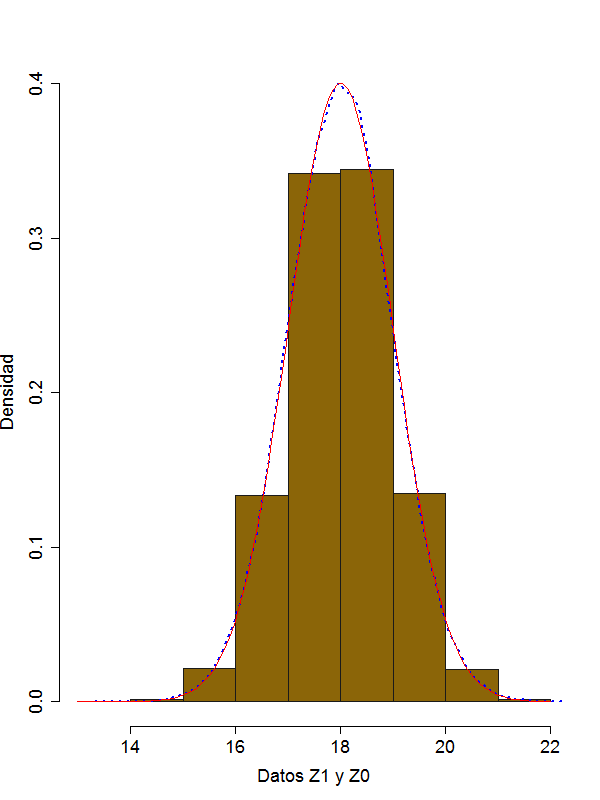
\includegraphics[width=0.3\textwidth]{BoxMuller.png}}%
\hfill
\caption{Densidad de las distribuciones generadas con el método de Box-Muller.}
\label{fig:foobar}
\end{figure}



\begin{figure}
\centering
\subcaptionbox{Distribución de frecuencia de la variable $Z_{0} $con solo una variable uniforme.}{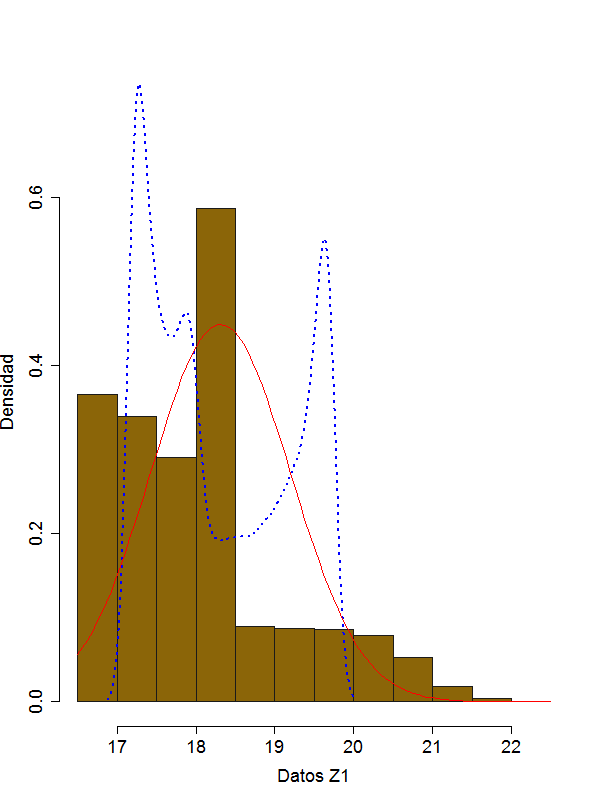
\includegraphics[width=0.5\textwidth]{BoxMuller_z1_variable_2.png}}%
\hfill
\subcaptionbox{Distribución de frecuencia de la variable $Z_{1}$con solo una variable uniforme.}{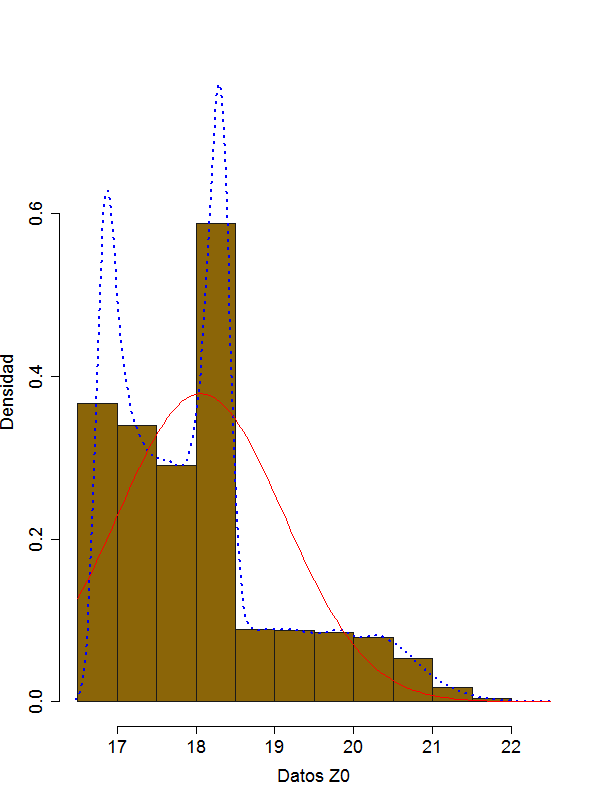
\includegraphics[width=0.5\textwidth]{BoxMuller_z1_variable_1.png}}%
\hfill

\caption{Distribución de frecuencia de la variables de Box-Muller con solo una variable uniforme.}
\label{fig:singlevariable}
\end{figure}










\printbibliography[title={Referencias}]
\end{document}
